\chapter{Résultats}

\section{Relèvement}
\label{respsih1}

Dans la figure \ref{az}, on peut observer la composante en $z$ de $\mathbf{a}$ dans le cylindre, lorsque $\alpha_1=0$ et $\alpha_0(x,y)=2\times v\times\left(1-\frac{x^2+y^2}{r^2}\right)$. Ce résultat a été obtenu avec le programme du chapitre \ref{impGradh1}. 

\begin{figure}[H]
\makebox[\textwidth][c]{
  \subfloat{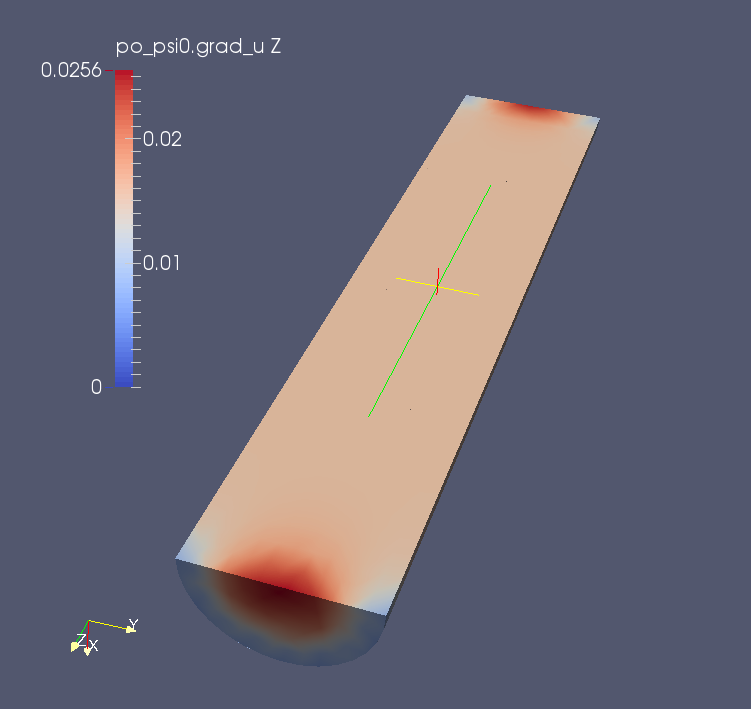
\includegraphics[scale=0.3]{az}}\ 
  \subfloat{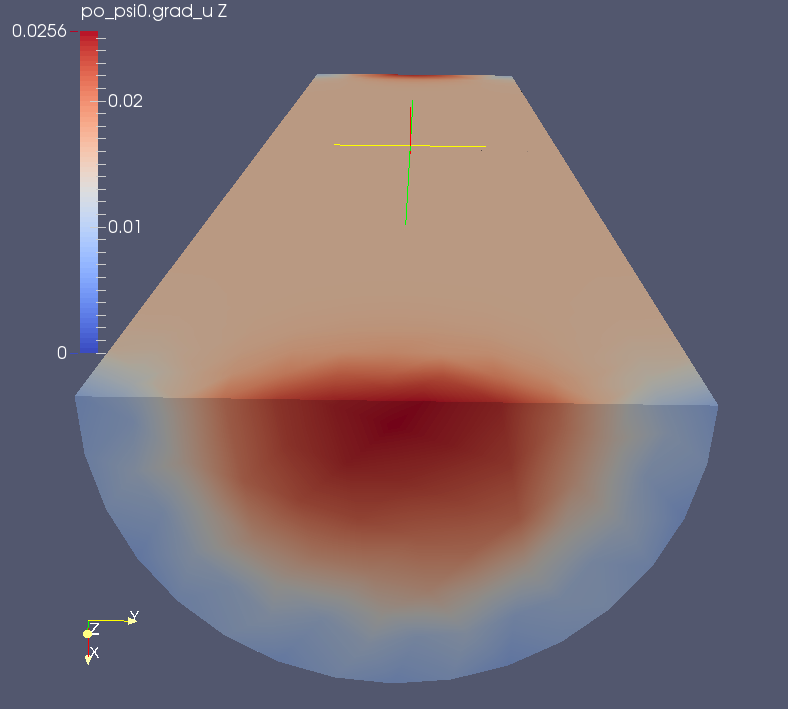
\includegraphics[scale=0.3]{az1}}
}
\caption{$\mathbf{a}=\grad\psi^0\in H(div)$}
\label{az}
\end{figure}

\section{Composante $z$}

\subsection{Expression analytique}

D'après \cite{Saks2005}, on a, pour un cylindre de longueur $l$ et de rayon $R$ :
\[
\lambda_\mathcal{K} = \sqrt{\frac{\rho_{k,j}^2}{R^2} + \frac{m^2\pi^2}{l^2}}
\]
où $\mathcal{K}=(k,j,m)$ est un multi-index et $\rho_{k,j}$ représente le j-ième zéro de la k-ième fonction de Bessel.\\
Dans notre cas, $l=0,5$ et $R=0,05$, d'où :\\
\begin{center}
\begin{tabular}{|*{8}{c|}}
\hline
k & j & m=1 & m=2 & m=3 & m=4 & m=5 & m=6\\
\hline
\multirow{3}{*}{0}
& 1 & 2352,703634&2471,138886&2668,530974&2944,879898&3300,185656&3734,44825\\
& 2 & 12228,08002&12346,51527&12543,90736&12820,25629&13175,56204&13609,82464\\
& 3 & 29994,08789&30112,52315&30309,91523&30586,26416&30941,56992&31375,83251\\
\hline
\multirow{3}{*}{1}
& 1 &5912,248374&6030,683626&6228,075714&6504,424638&6859,730396&7293,99299\\
& 2 &19726,93576&19845,37101&20042,7631&20319,11203&20674,41778&21108,68038\\
& 3 &41439,51932&41557,95457&41755,34666&42031,69558&42387,00134&42821,26393\\ \hline
\multirow{3}{*}{2}
& 1 &10589,23336&10707,66861&10905,0607&11181,40963&11536,71538&11970,97798\\
& 2 &28379,18075&28497,61601&28695,00809&28971,35702&29326,66278&29760,92537\\
& 3 &54047,37923&54165,81449&54363,20657&54639,5555&54994,86126&55429,12385\\
\hline
\multirow{3}{*}{3}
& 1 &16322,25923&16440,69449&16638,08657&16914,4355&17269,74126&17704,00385\\
& 2 &38150,32682&38268,76207&38466,15416&38742,50308&39097,80884&39532,07143\\
& 3 &67797,65083&67916,08609&68113,47817&68389,8271&68745,13286&69179,39545\\
\hline
\multirow{3}{*}{4}
& 1 &23072,39717&23190,83243&23388,22451&23664,57344&24019,8792&24454,14179\\
& 2 &49010,51285&49128,94811&49326,34019&49602,68912&49957,99488&50392,25747\\
& 3 &82666,98092&82785,41617&82982,80826&83259,15718&83614,46294&84048,72553\\
\hline
\end{tabular}
\end{center}

Il montre aussi que :
\[
g_\mathcal{K}^z(r,\theta,z) = \frac{\sqrt{2}}{\sqrt{l\pi}R|J_k'\left(\rho_{k,j}\frac{r}{R}\right)}exp(ik\theta)sin\left(\frac{m\pi}{l}z\right)
\]

\subsection{Sans relèvement}
\label{resZSR}

On va ici utiliser l'implémentation présenté dans la section \ref{impZSR}.

\subsubsection{Modes propres}
On obtient les valeurs propres suivantes, où l'on voit que $m=1$ pour toutes les valeurs propres, et que celles ne correspondant pas à la fonction 0 de Bessel, apparaissent deux fois, cela est dû à la symétrie du cylindre.\\
D'autre part, on voit qu'à partir d'un certain moment, les valeurs propres ne correspondent plus aux valeurs analytiques et leur divergence explose. Cela est dû à la taille du maillage, trop grossière pour calculer des modes aux variations de plus en plus fines.\\
\begin{align*}
\bm{\lambda^2_{0,1,1}=\Lambda_0} &\bf{= 2329.47}	&\int\div\bm{h} &= 1.94208e-17	&||\div\bm{h}|| &= 0.0983456\\
\lambda^2_{1,1,1}=\Lambda_1 &= 5917.22	&\int\div\bm{h} &= 3.17129e-18	&||\div\bm{h}|| &= 0.296662\\
\lambda^2_{1,1,1}=\Lambda_2 &= 5917.43	&\int\div\bm{h} &= -3.4708e-17	&||\div\bm{h}|| &= 0.299039\\
\lambda^2_{2,1,1}=\Lambda_3 &= 10644.7	&\int\div\bm{h} &= 2.20627e-17	&||\div\bm{h}|| &= 0.683934\\
\lambda^2_{2,1,1}=\Lambda_4 &= 10647.4	&\int\div\bm{h} &= 2.89804e-17	&||\div\bm{h}|| &= 0.688444\\
\bm{\lambda^2_{0,2,1}=\Lambda_5} &\bf{= 12312.1}	&\int\div\bm{h} &= -1.04863e-16	&||\div\bm{h}|| &= 0.954444\\
\lambda^2_{3,1,1}=\Lambda_6 &= 16473	&\int\div\bm{h} &= -1.28681e-17	&||\div\bm{h}|| &= 1.23079\\
\lambda^2_{3,1,1}=\Lambda_7 &= 16474.4	&\int\div\bm{h} &= -2.9924e-17	&||\div\bm{h}|| &= 1.22237\\
\lambda^2_{1,2,1}=\Lambda_8 &= 19976.6	&\int\div\bm{h} &= -5.4515e-17	&||\div\bm{h}|| &= 1.8095\\
&\vdots & &\vdots & &\vdots\\
\lambda^2_{?,?,?}=\Lambda_{35} &= 51355.4	&\int\div\bm{h} &= 1.14817e-16	&||\div\bm{h}|| &= 7.14748\\
\lambda^2_{?,?,?}=\Lambda_{36} &= 54891.3	&\int\div\bm{h} &= 1.21431e-17	&||\div\bm{h}|| &= 50.2826\\
\lambda^2_{?,?,?}=\Lambda_{37} &= 55565.9	&\int\div\bm{h} &= -2.43729e-16	&||\div\bm{h}|| &= 52.281\\
\lambda^2_{?,?,?}=\Lambda_{38} &= 55976.2	&\int\div\bm{h} &= -1.73906e-16	&||\div\bm{h}|| &= 58.8682\\
\lambda^2_{?,?,?}=\Lambda_{39} &= 56447.3	&\int\div\bm{h} &= 1.50813e-16	&||\div\bm{h}|| &= 59.4463\\
\lambda^2_{?,?,?}=\Lambda_{40} &= 57302.4	&\int\div\bm{h} &= 4.13081e-17	&||\div\bm{h}|| &= 40.4527\\
\lambda^2_{?,?,?}=\Lambda_{41} &= 57360.6	&\int\div\bm{h} &= -3.61581e-17	&||\div\bm{h}|| &= 36.7049\\
\lambda^2_{?,?,?}=\Lambda_{42} &= 57614.4	&\int\div\bm{h} &= -8.2833e-17	&||\div\bm{h}|| &= 44.0287\\
\lambda^2_{?,?,?}=\Lambda_{43} &= 57825.8	&\int\div\bm{h} &= 1.47451e-16	&||\div\bm{h}|| &= 58.9588\\
\lambda^2_{?,?,?}=\Lambda_{44} &= 58151.4	&\int\div\bm{h} &= -9.36751e-17	&||\div\bm{h}|| &= 62.1296
\end{align*}

Les modes correspondant aux trois premiers zéros de la fonction 0 de Bessel sont présenté dans la figure suivante, avec un autre mode où l'on voit que ces fonctions ne dépendent pas de $\theta$ contrairement aux autres :
\begin{figure}[H]
	\makebox[\textwidth][c]{
		\subfloat[mode 0]{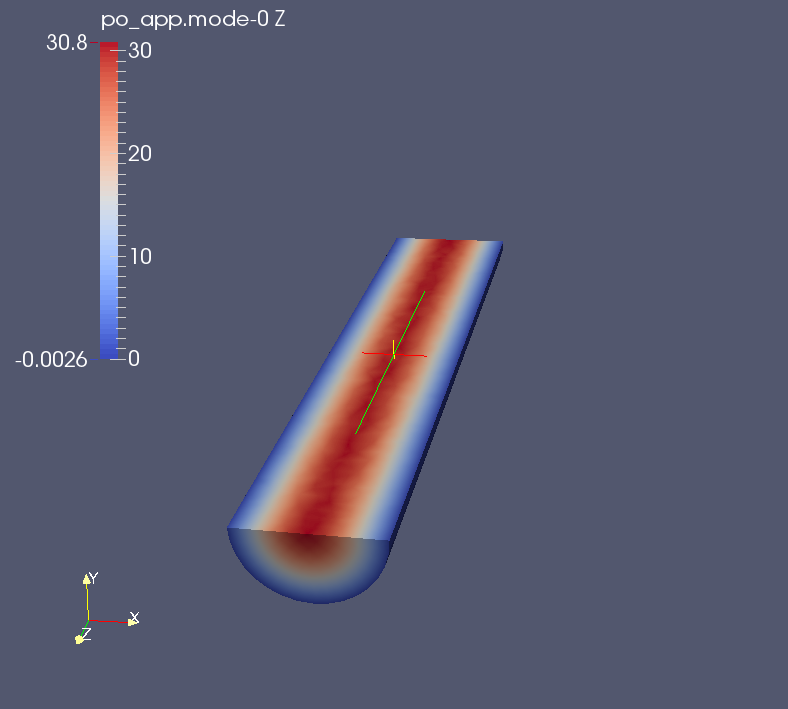
\includegraphics[scale=0.3]{modeZ-0}}\ 
		\subfloat[mode 5]{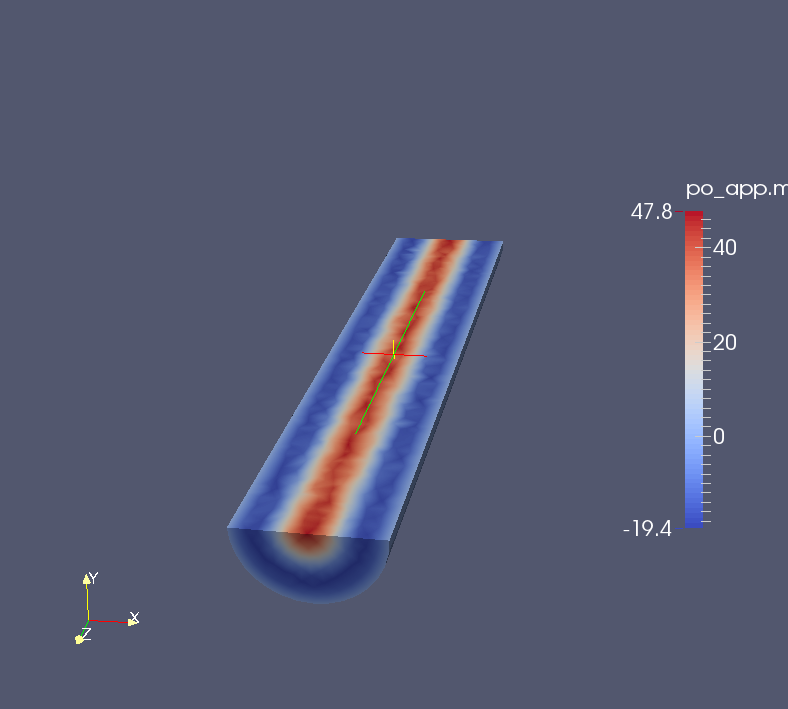
\includegraphics[scale=0.3]{modeZ-5}}
	}\\
	\makebox[\textwidth][c]{
		\subfloat[mode 14]{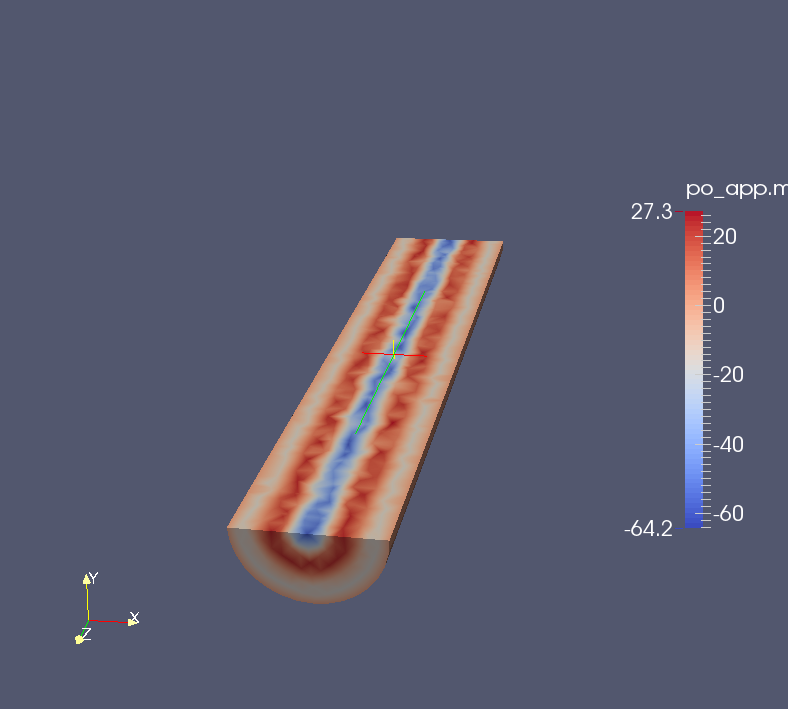
\includegraphics[scale=0.3]{modeZ-14}}\ 
		\subfloat[mode 16]{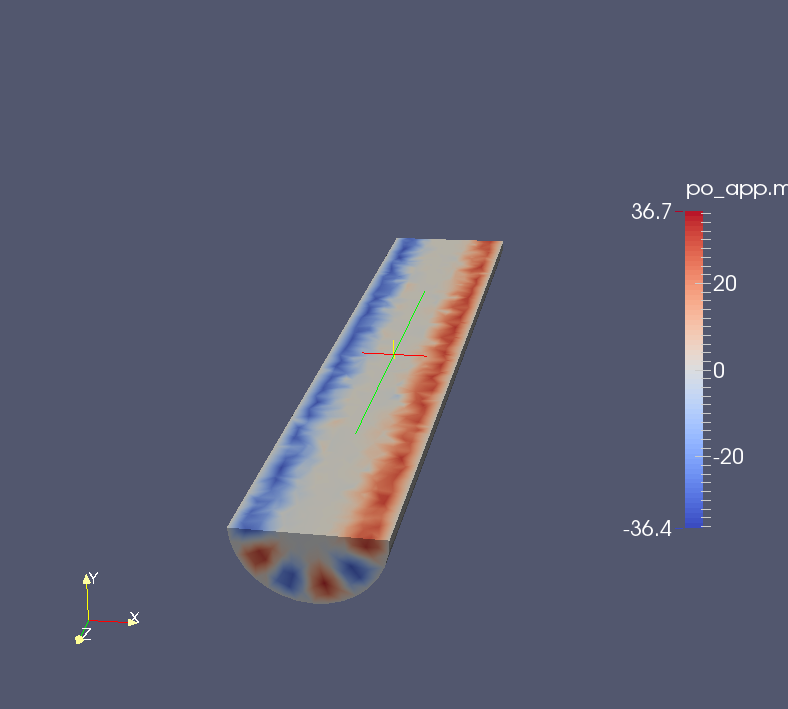
\includegraphics[scale=0.3]{modeZ-16}}
	}
	\caption{composante z des fonctions propres}
	\label{resultats}
\end{figure}

\subsubsection{Problème spectral}
\label{resZSRPS}

En utilisant \ref{impZPS} et $\bm{f}=(0,0,1)$ et $\alpha_2=\frac{2\times v}{R^2}$, on obtient les coefficients suivants :
\begin{align*}
\bf{d_{0}} &\bf{= 0.00242664} & d_{1} &= -5.72621e-05\\
d_{2} &= -2.79554e-05 & d_{3} &= 1.17409e-06\\
d_{4} &= 2.4402e-05 & \bf{d_{5}} &\bf{= -0.000211458}\\
d_{6} &= -7.79286e-06 & d_{7} &= -6.61541e-07\\
d_{8} &= -6.61893e-07 & d_{9} &= -4.8829e-06\\
d_{10} &= 1.91622e-05 & d_{11} &= 1.27225e-07\\
d_{12} &= 3.64327e-06 & d_{13} &= -1.34974e-06\\
\bf{d_{14}} &\bf{= 6.02757e-05} & d_{15} &= -3.67763e-07
\end{align*}

Où les coefficients en gras correspondent aux valeurs des fonctions 0 de Bessel. Ce sont les seules qui ne sont pas nuls, et on voit que leur poids diminue rapidement.\\
En additionnant les vecteurs propres multipliés par leur coefficient, on arrive au vecteur vitesse suivant :

\begin{figure}[H]
\makebox[\textwidth][c]{
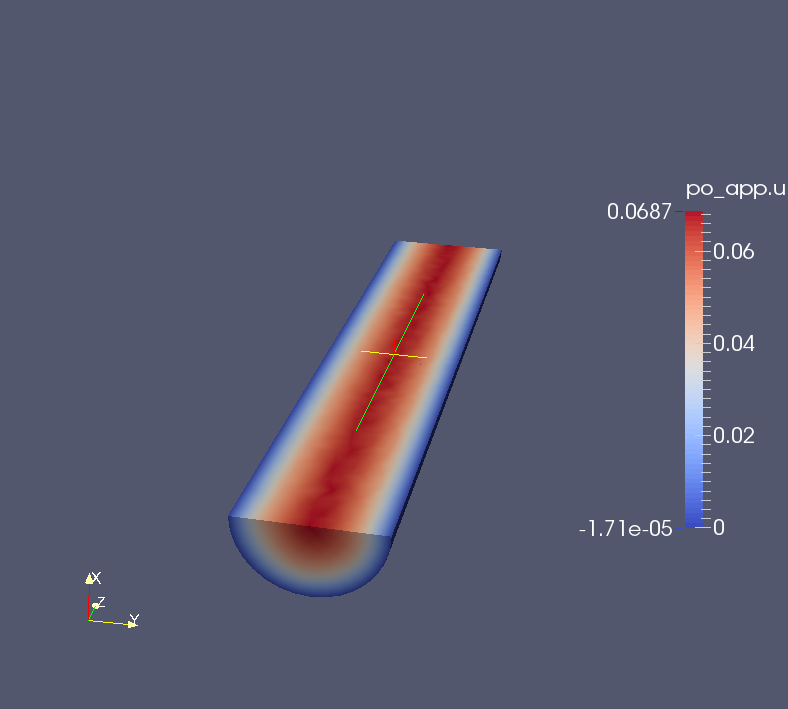
\includegraphics[scale=0.5]{vZ}}
\caption{$\bm{v}$ avec 100 modes propres}
\end{figure}

A un coefficient d'adimensionnement près, les résultats sont ceux recherchés.\\

Mais la formulation mathématique de cette méthode n'est pas rigoureuse, et il y a de fortes chances que l'on ne puisse pas utiliser cette méthode dans d'autres cas que le cylindre. De plus, on perd le contrôle de $\alpha_0$ et $\alpha_1$.

\subsection{Avec relèvement}
\label{resZAR}

\subsubsection{Modes propres}

Ici, les valeurs propres correspondent bien à toutes les valeurs analytiques que R. Saks trouvent, de plus, on a bien plus de valeurs propres cohérentes bien que la taille de maillage soit la même.\\
Par contre, on a encore les valeurs qui apparaissent en double dû à la symétrie du cylindre.\\
Il faut noter que la divergence augmente linéairement et est égale environ à $m\times 2\pi$.\\

\begin{align*}
\lambda^2_{0,1,1} = \Lambda_{0} &= 2369	& \int\div\bm{g} &= -1.60651e-09	& ||\div\bm{g}|| &= 6.24909\\
\lambda^2_{0,1,2} = \Lambda_{1} &= 2487.46	& \int\div\bm{g} &= 7.32721e-07	& ||\div\bm{g}|| &= 12.4931\\
\lambda^2_{0,1,3} = \Lambda_{2} &= 2684.89	& \int\div\bm{g} &= 4.90275e-09	& ||\div\bm{g}|| &= 18.7299\\
\lambda^2_{0,1,4} = \Lambda_{3} &= 2961.33	& \int\div\bm{g} &= 1.74436e-06	& ||\div\bm{g}|| &= 24.9565\\
\lambda^2_{0,1,5} = \Lambda_{4} &= 3316.78	& \int\div\bm{g} &= 1.10662e-08	& ||\div\bm{g}|| &= 31.1678\\
\lambda^2_{0,1,6} = \Lambda_{5} &= 3751.28	& \int\div\bm{g} &= -3.31484e-06	& ||\div\bm{g}|| &= 37.3597\\
\lambda^2_{0,1,7} = \Lambda_{6} &= 4264.86	& \int\div\bm{g} &= 1.97088e-08	& ||\div\bm{g}|| &= 43.5285\\
\lambda^2_{0,1,8} = \Lambda_{7} &= 4857.65	& \int\div\bm{g} &= 5.72063e-06	& ||\div\bm{g}|| &= 49.6785\\
\lambda^2_{0,1,9} = \Lambda_{8} &= 5529.66	& \int\div\bm{g} &= 3.31517e-08	& ||\div\bm{g}|| &= 55.7955\\
\lambda^2_{1,1,1} = \Lambda_{9} &= 5956.95	& \int\div\bm{g} &= -5.20023e-09	& ||\div\bm{g}|| &= 6.20444\\
&\vdots & &\vdots & &\vdots\\
\lambda^2_{1,1,9} = \Lambda_{30} &= 9124.64	& \int\div\bm{g} &= -1.66897e-07	& ||\div\bm{g}|| &= 55.404\\
\lambda^2_{1,1,10} = \Lambda_{31} &= 9877.82	& \int\div\bm{g} &= -7.9746e-08	& ||\div\bm{g}|| &= 61.4882\\
\lambda^2_{1,1,10} = \Lambda_{32} &= 9878.29	& \int\div\bm{g} &= 5.9413e-08	& ||\div\bm{g}|| &= 61.4728\\
\lambda^2_{0,1,14} = \Lambda_{33} &= 10084.8	& \int\div\bm{g} &= -2.07731e-05	& ||\div\bm{g}|| &= 85.9147\\
\lambda^2_{2,1,1} = \Lambda_{34} &= 10685.8	& \int\div\bm{g} &= 9.04227e-08	& ||\div\bm{g}|| &= 6.19571\\
\lambda^2_{2,1,1} = \Lambda_{35} &= 10688.2	& \int\div\bm{g} &= 1.56108e-08	& ||\div\bm{g}|| &= 6.28396\\
\lambda^2_{1,1,11} = \Lambda_{36} &= 10711	& \int\div\bm{g} &= -2.3174e-07	& ||\div\bm{g}|| &= 67.4732\\
\lambda^2_{1,1,11} = \Lambda_{37} &= 10711.4	& \int\div\bm{g} &= -4.91277e-08	& ||\div\bm{g}|| &= 67.535\\
\lambda^2_{2,1,2} = \Lambda_{38} &= 10804.7	& \int\div\bm{g} &= 1.65283e-07	& ||\div\bm{g}|| &= 12.3054\\
\lambda^2_{2,1,2} = \Lambda_{39} &= 10806.9	& \int\div\bm{g} &= 3.99449e-08	& ||\div\bm{g}|| &= 12.3059
\end{align*}

Les modes correspondants à $\lambda_{0,1,1}$, $\lambda_{0,1,4}$, $\lambda_{1,1,1}$ et $\lambda_{2,1,1}$ sont présentés dans la figure suivante :
\begin{figure}[H]
	\makebox[\textwidth][c]{
		\subfloat[mode 0]{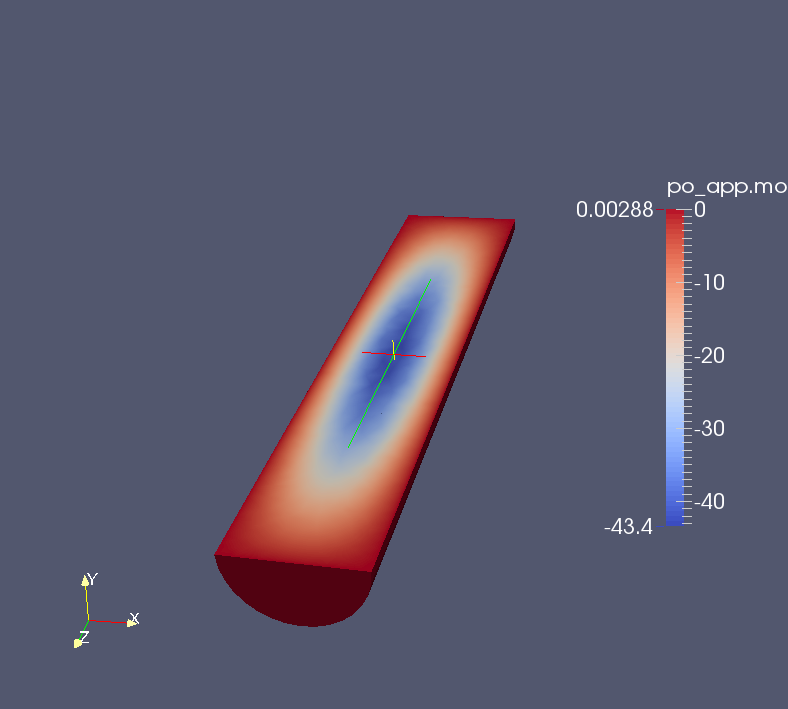
\includegraphics[scale=0.3]{modeZAR-0}}\ 
		\subfloat[mode 3]{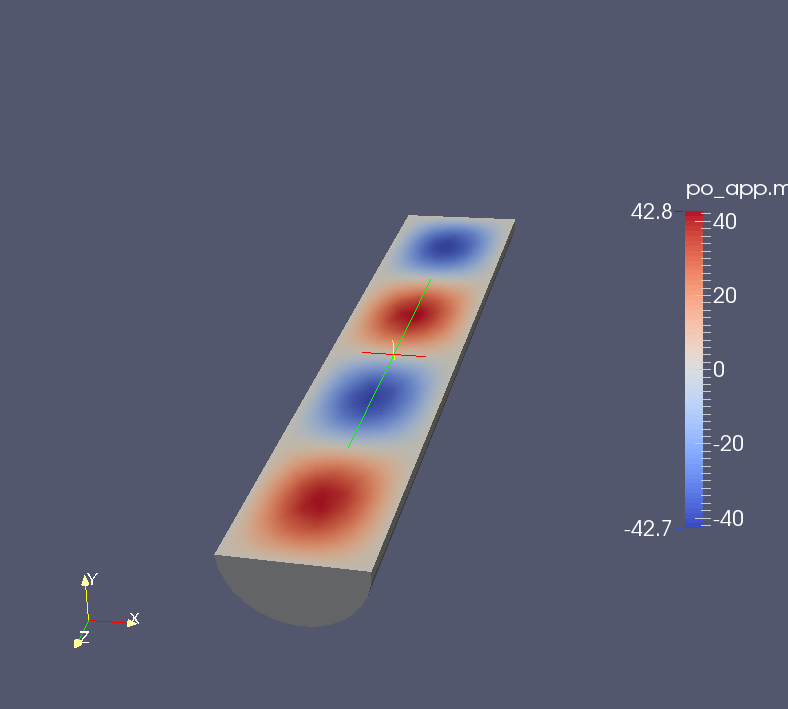
\includegraphics[scale=0.3]{modeZAR-3}}
	}\\
	\makebox[\textwidth][c]{
		\subfloat[mode 9]{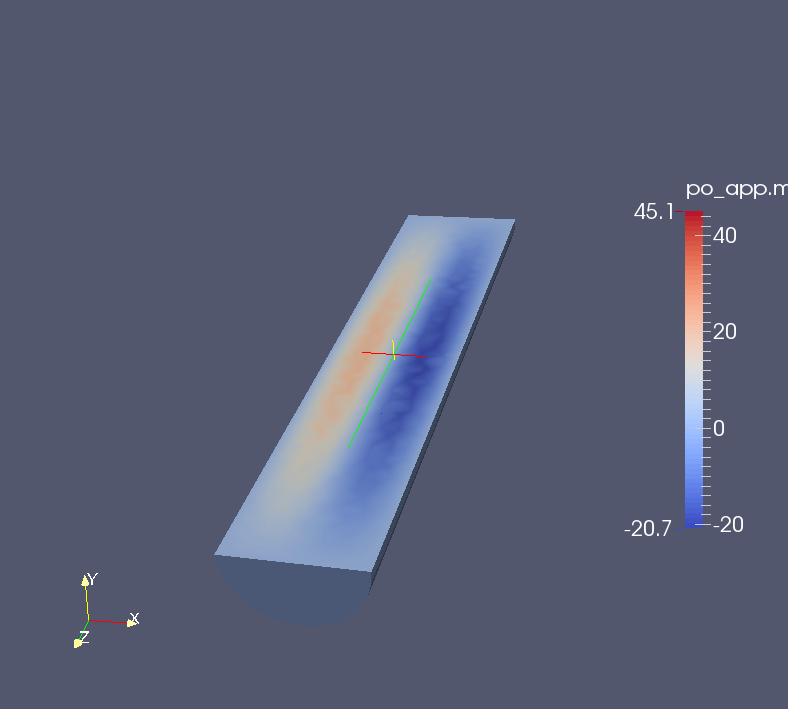
\includegraphics[scale=0.3]{modeZAR-9}}\ 
		\subfloat[mode 34]{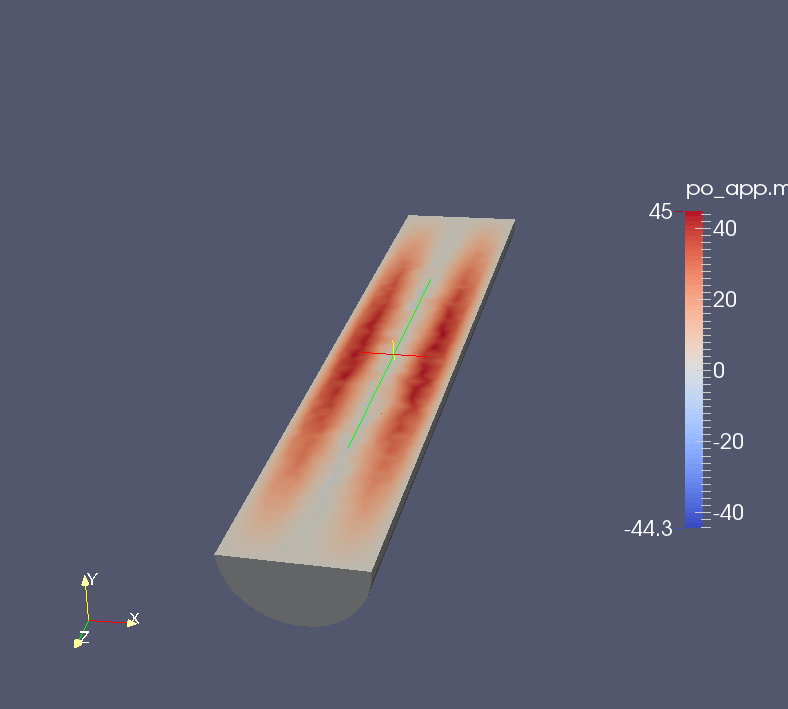
\includegraphics[scale=0.3]{modeZAR-34}}
	}
	\caption{composante z des fonctions propres}
	\label{modesZAR}
\end{figure}

\subsubsection{Problème spectral}

En utilisant les mêmes paramètres que dans \ref{resZSRPS}, on obtient les coefficients suivants :
\begin{align*}
c_{0} &= -0.00162348 & c_{1} &= 2.76514e-05\\
c_{2} &= 0.000461607 & c_{3} &= 0.000621154\\
c_{4} &= 0.000261723 & c_{5} &= -0.000181696\\
c_{6} &= -6.11957e-05 & c_{7} &= -3.59883e-05\\
c_{8} &= 8.39453e-05 & c_{9} &= 2.42786e-05\\
c_{10} &= 2.29969e-07 & c_{11} &= -8.20664e-05\\
c_{12} &= 1.98117e-05 & c_{13} &= -0.000165568\\
c_{14} &= -1.08967e-05 & c_{15} &= 4.07849e-05
\end{align*}

Ce qui correspond à la vitesse présenté dans la figure suivante :
\begin{figure}[H]
\makebox[\textwidth][c]{
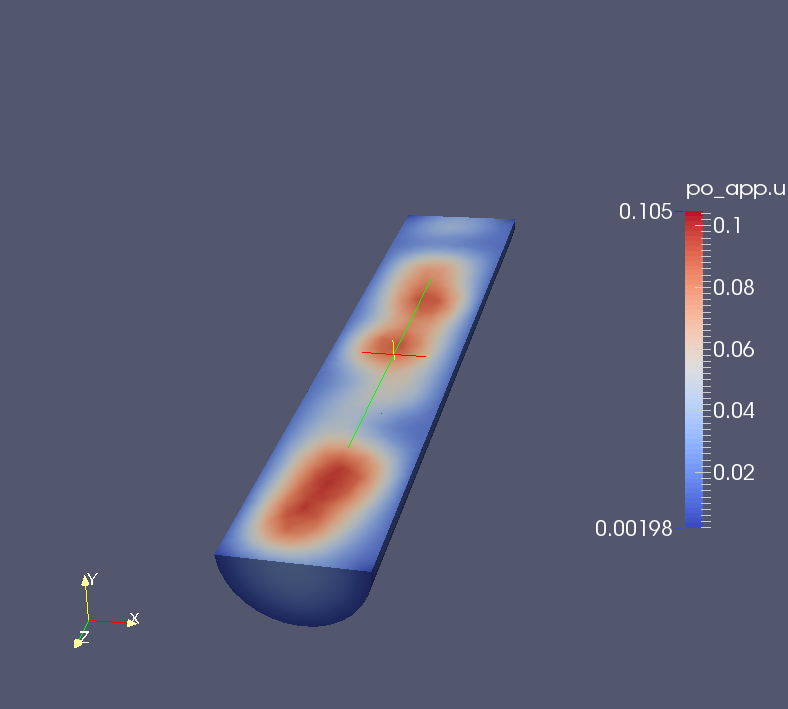
\includegraphics[scale=0.5]{vZAR}}
\caption{$\bm{v}$ avec 40 modes propres}
\end{figure}
Il y a évidemment des problèmes, cela peut venir soit du fait que certains paramètres ne soient pas valides, soit du fait que l'hypothèse qui consiste à dire que $\bm{g_i}=(0,0,g_i^z)$ est fausse.\\

Pour ma part, je pense que l'on ne peut pas prendre $\bm{g_i}$ sous cette forme, en effet si $\bm{v}$ est bien sous cette forme dans le cylindre, $\bm{a}$ ne l'est pas, et donc $\bm{u}$ ne devrait pas l'être non plus.

\section{Cas général}

\subsection{Modes propres}

\subsection{Problème spectral}

\iffalse

Pour mémoire, voici les résultats de différents modes obtenus avec freefem++.\\

\begin{figure}[H]
\makebox[\textwidth][c]{
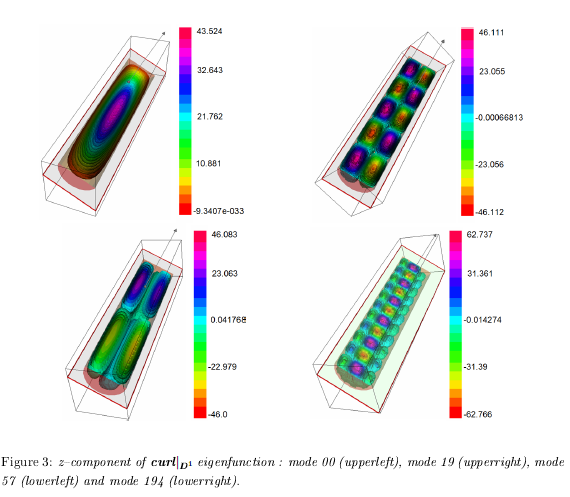
\includegraphics[scale=1]{Exemple_de_modes}}
\end{figure}

On peut voir les mêmes modes obtenus avec Feel++ dans la figure \ref{modes}.\\

\begin{figure}[H]
	\makebox[\textwidth][c]{
		\subfloat[mode00]{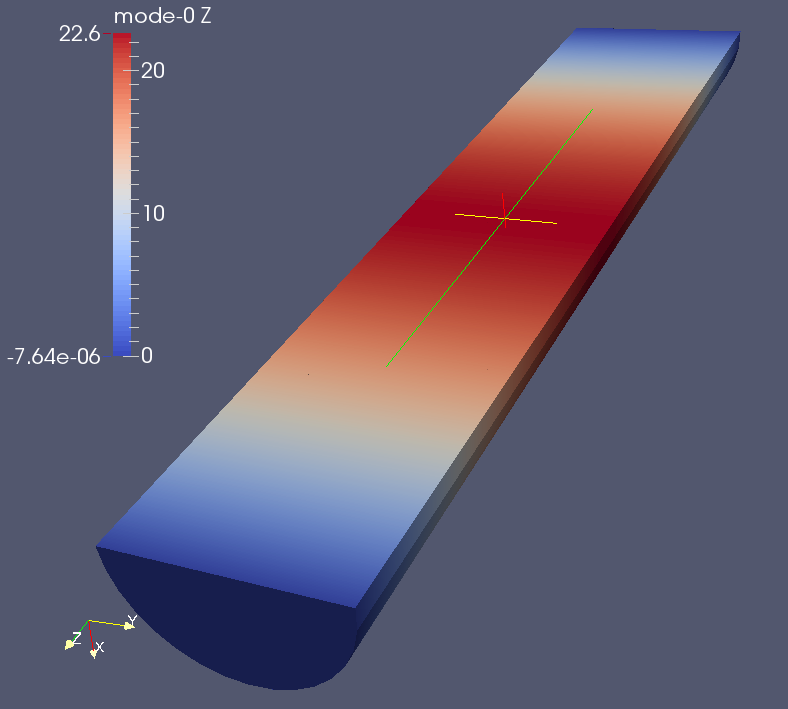
\includegraphics[scale=0.3]{mode00}}\ 
		\subfloat[mode19]{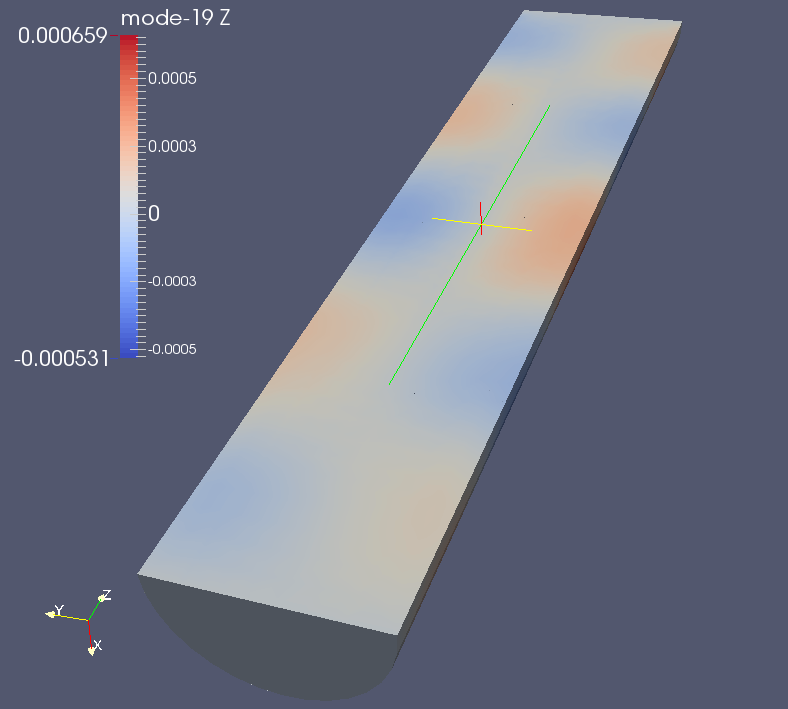
\includegraphics[scale=0.3]{mode19}}
	}\\
	\makebox[\textwidth][c]{
		\subfloat[mode57]{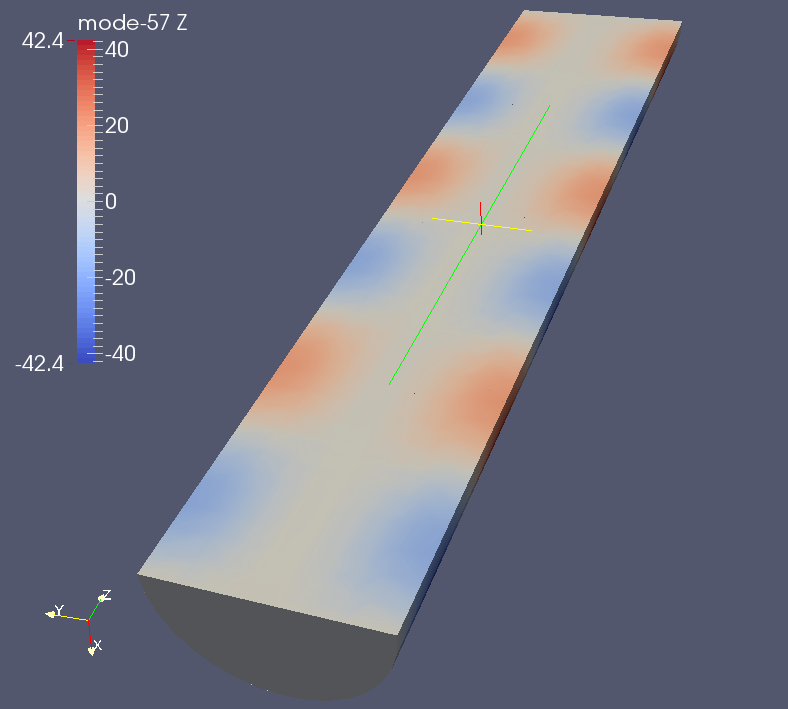
\includegraphics[scale=0.3]{mode57}}\ 
		\subfloat[mode194]{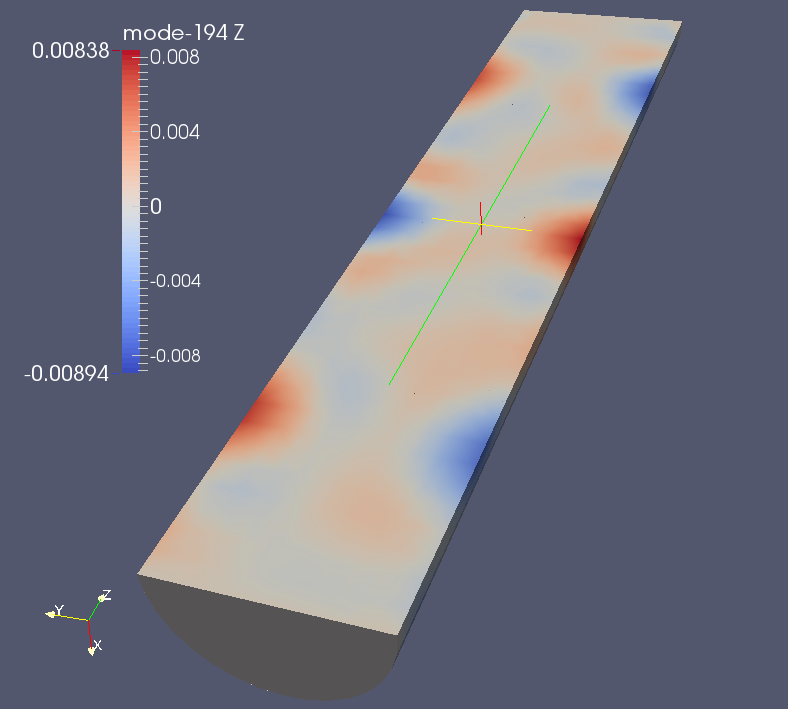
\includegraphics[scale=0.3]{mode194}}
	}
	\caption{composante z des fonctions propres}
	\label{modes}
\end{figure}

\fi


%%% Local Variables:
%%% TeX-master: "../report.tex"
%%% End:
